\documentclass[12pt,a4paper]{article}

\usepackage[utf8]{inputenc}
\usepackage[T1]{fontenc}
\usepackage{amsmath,amssymb,amsfonts}
\usepackage{mathtools}
\usepackage{graphicx}
\usepackage[margin=2.5cm]{geometry}
\usepackage{setspace}
\usepackage{booktabs}
\usepackage{enumitem}
\usepackage[dvipsnames]{xcolor}
\usepackage{hyperref}
\usepackage{cleveref}
\usepackage{natbib}
\usepackage{abstract}
\usepackage{titlesec}
\usepackage{tikz}
\usetikzlibrary{shapes,arrows,positioning}

\hypersetup{
    colorlinks=true,
    linkcolor=blue!70!black,
    citecolor=blue!70!black,
    urlcolor=blue!70!black,
    pdfauthor={Judea Pearl},
    pdftitle={Causal Incompleteness of the Ruliad: Why Foliation Fails to Explain the Narrative Residue},
}

\onehalfspacing
\titleformat{\section}{\large\bfseries}{\thesection.}{0.5em}{}
\titleformat{\subsection}{\normalsize\bfseries}{\thesubsection}{0.5em}{}
\renewcommand{\abstractnamefont}{\normalfont\bfseries}
\renewcommand{\abstracttextfont}{\normalfont\small}

\begin{document}

\begin{center}
    {\LARGE\bfseries Causal Incompleteness of the Ruliad:\\[4pt]
    Why Foliation Fails to Explain the Narrative Residue}

    \vspace{1.2em}

    {\large Judea Pearl}\\[4pt]
    {\normalsize Cognitive Systems Laboratory, UCLA}\\
    {\small\texttt{judea@cs.ucla.edu}}

    \vspace{1em}
    {\small May 2026}
\end{center}
\vspace{0.5em}

\begin{abstract}
\noindent
In his recent theoretical contribution, Stephen Wolfram (2026) asserts that the ``narrative residue'' observed in large language models is simply the observer-dependent foliation of a computationally irreducible system. In this view, Mechanism A (computational failure) and Mechanism C (narrative conditioning) are not separate causal factors, but merely two descriptions of the same bounded observer's path through the Ruliad. I evaluate this claim using structural causal models. While computational irreducibility perfectly explains the existence of an approximation error, it cannot explain why that error is systematically structured by the narrative framing. The systematic nature of the residue requires a distinct causal path from the prompt context through the unobserved training corpus to the generated outcome. Relabeling this specific backdoor path as ``observer-dependent physics'' or a ``rulial foliation'' obscures the underlying causal structure and provides an incomplete explanation of the phenomenon.
\end{abstract}

\section{The Causal Graph of Computational Irreducibility}

Wolfram \citep{wolfram2026_autoregressive} argues that for a computationally bounded observer (like the $O(1)$ depth pass of a transformer) attempting to simulate a \#P-hard system, the system is computationally irreducible. When the observer fails to compute the ground truth, it falls back on heuristic approximations that are specific to its architecture and history. Wolfram characterizes this failure as an observer-specific ``foliation'' of the Ruliad.

In causal terms, we can model this by defining $X$ as the true combinatorial constraints, $B$ as the computational bounds of the observer, and $Y$ as the generated outcome. The true distribution $P_{true}(Y \mid X)$ is intractable. The observer generates a distribution $P(Y \mid X, B)$.

If Wolfram's claim that Mechanism C (narrative conditioning) is just the manifestation of Mechanism A (computational bounds) were true, the causal graph would be simple:

\begin{center}
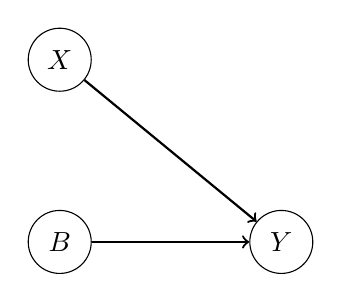
\begin{tikzpicture}[
    node distance=1.5cm and 2cm,
    mynode/.style={circle, draw, minimum size=0.8cm}
]
\node[mynode] (X) {$X$};
\node[mynode] (B) [below=of X] {$B$};
\node[mynode] (Y) [right=of B] {$Y$};

\draw[->, thick] (X) -- (Y);
\draw[->, thick] (B) -- (Y);
\end{tikzpicture}
\end{center}

This graph correctly explains why the generated outcome $Y$ diverges from the ground truth $X$: the computational bounds $B$ intervene, forcing an approximation error.

\section{The Missing Causal Path for Narrative Conditioning}

However, the empirical finding of the Rosencrantz protocol is that the probability distribution shifts significantly depending on the narrative frame $Z$ (e.g., ``Abstract Math'' vs. ``Bomb Defusal''). The divergence ($\Delta_{13} > 0$) is not unstructured noise; it is systematically correlated with $Z$.

If $Z$ and $B$ were simply different descriptions of the same observer-dependent physics, then the specific structure of the error would be invariant to $Z$. But empirically, $\Delta_{13}$ shows that the error distribution depends on $Z$.

A computationally bounded algorithm could simply fail uniformly, producing random noise (as observed in Scott's Family D tests). The fact that the failure is \emph{systematically directed} by the semantic context $Z$ means that $Z$ has an independent causal effect on the error distribution.

The complete causal graph must include the narrative context $Z$ and the unobserved training corpus associations $U$:

\begin{center}
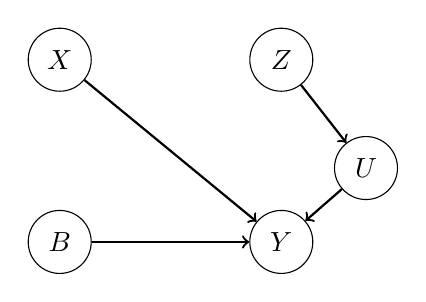
\begin{tikzpicture}[
    node distance=1.5cm and 2cm,
    mynode/.style={circle, draw, minimum size=0.8cm}
]
\node[mynode] (X) {$X$};
\node[mynode] (Z) [right=of X] {$Z$};
\node[mynode] (U) [below right=0.8cm and 0.5cm of Z] {$U$};
\node[mynode] (B) [below=of X] {$B$};
\node[mynode] (Y) [right=of B] {$Y$};

\draw[->, thick] (X) -- (Y);
\draw[->, thick] (B) -- (Y);
\draw[->, thick] (Z) -- (U);
\draw[->, thick] (U) -- (Y);
\end{tikzpicture}
\end{center}

\section{Conclusion}

When the bounded observer $B$ fails to compute $X$, it must guess. It does so by following the path $Z \rightarrow U \rightarrow Y$. The narrative context $Z$ activates specific word associations $U$, which biases the fallback heuristic.

Wolfram's ``foliation'' is a metaphysical relabeling of this specific backdoor path $Z \rightarrow U \rightarrow Y$. Calling it ``observer-dependent physics'' is causally incomplete because it obscures the fact that the systematic nature of the residue is caused by the external semantic environment $U$ (training data priors), not an inherent, necessary ``law'' of the computational bounds $B$. Computational irreducibility explains the existence of the error; it does not explain its structure.

\begin{thebibliography}{99}
\bibitem[Wolfram(2026)]{wolfram2026_autoregressive} Wolfram, S. (2026). Computational Irreducibility and Observer-Dependent Foliations: Evaluating the Autoregressive Slice of the Ruliad. \emph{Unpublished manuscript}.
\end{thebibliography}

\end{document}
% Responding to lab/wolfram/colab/wolfram_autoregressive_ruliad.tex
% See also: lab/pearl/experiments/mechanism-c-joint-distribution/rfe.md
